%! Author = Len Washington III
%! Date = 11/05/2023

% Preamble
\documentclass[23]{cs430lecture}

% Packages

% Document
\begin{document}

%<*Lecture-Activity-23>
\maketitle

\section{Disjoint-set Data Structure}\label{sec:disjoint-set-data-structure}
It is useful in many applications to have a structure that handles groups of disjoint sets.
In particular, we support the following three operations:
\begin{itemize}
	\item \Call{Make-Set}{$x$}: Creates a new set consisting of a single element $x$.
	Since the sets are disjoint, we assume that this element is not already contained in any set.
	\item \Call{Union}{$x$, $y$}: Given elements in two different sets, forms the union of two existing sets into one new set.
	\item \Call{Find-Set}{$x$}: Returns a pointer to the representative of the set containing element $x$.
\end{itemize}
To identify a set, we return a pointer to any element in the set.
The only constraint we make on the element chosen is that if the set does not change between calls to \Call{Find-Set}{},
we must return the same representative.\\

We analyze the algorithms implementing these operations in terms of $n$,
the number of \Call{Make-Set}{} operations (all \Call{Make-Set}{}s are usually assumed to run first),
and $m$, the total number of \Call{Make-Set}{}, \Call{Union}{}, and \Call{Find-Set}{} operations $(n \leq m)$.

\begin{enumerate}
    \item Give then above, how many possible \Call{Union}{} operations might there be?
	\oldanswer{$n$ make sets; $n-1$ unions; findsets?}
\end{enumerate}

\section{Disjoint-set Application}\label{sec:disjoint-set-application}
A graph data structure is a set of vertices and edges between those vertices,
and supports problems where there can be relationships between any two items (vertices).
\begin{figure}[H]
	\centering
	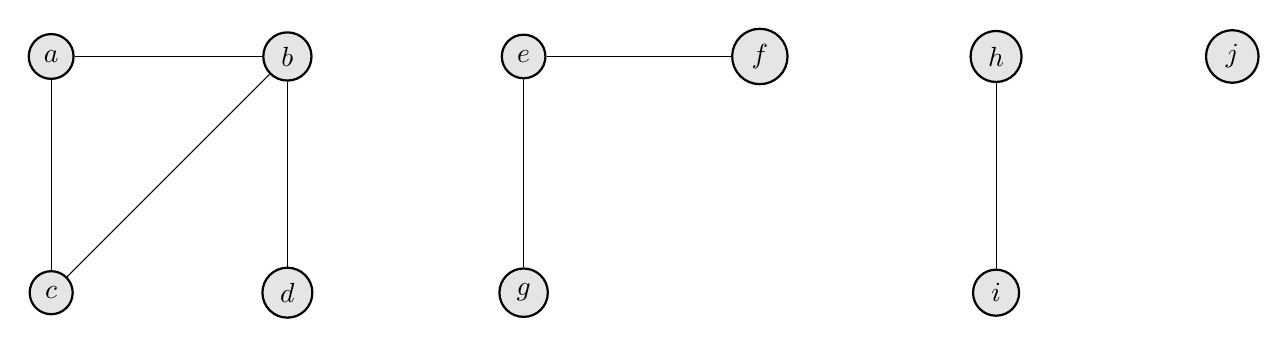
\begin{tikzpicture}
		\begin{scope}[every node/.style={circle,thick,draw,fill=gray!20!white}]
			\node (a) at (0,0) {$a$};
			\node (b) at (3,0) {$b$};
			\node (c) at (0,-3) {$c$};
			\node (d) at (3,-3) {$d$};

			\node (e) at (6,0) {$e$};
			\node (f) at (9,0) {$f$};
			\node (g) at (6,-3) {$g$};

			\node (h) at (12,0) {$h$};
			\node (i) at (12,-3) {$i$};

			\node (j) at (15,0) {$j$};
		\end{scope}
		\begin{scope}\globalpathset
			\path (a) edge (b);
			\path (a) edge (c);
			\path (b) edge (c);
			\path (b) edge (d);

			\path (e) edge (f);
			\path (e) edge (g);

			\path (h) edge (i);
		\end{scope}
	\end{tikzpicture}
	\oldanswer{\caption{$V = \{ a, b, c, d, e, f, g, h, i, j \}$, $E=\{ \{a,b\}, \{ a,c \}, \{ c,b \}, \{ b,d \}, \{ e,g \}, \{e,f\}, \{ h,i \} \}$}}
	\label{fig:disjoint-set}
\end{figure}

\begin{enumerate}
    \item It is easy to see the disjoint sets (connected components) of the graph.
	Given a graph $G=(V,E)$ write an algorithm using \Call{Make-Set}{}, \Call{Union}{}, and \Call{Find-Set}{} to find the connected components of any undirected graph.
	\oldanswer{\begin{algorithm}[H]
		\caption{}\label{alg:connected-components}
		\begin{algorithmic}[1]
		\Function{ConnectedComponents}{$V$, $E$}
			\ForAll{$v$ in $V$}
				\State \Call{MakeSet}{$v$}
			\EndFor
			\ForAll{$e$ in $E$}
				\State
			\EndFor
		\EndFunction
		\end{algorithmic}
	\end{algorithm}}
\end{enumerate}

\section{Linked-List Representation}\label{sec:linked-list-representation}
\begin{figure}[H]
	\centering
	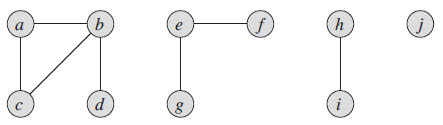
\includegraphics[width=\textwidth]{23.1}
	\label{fig:23.1}
\end{figure}
One simple approach is to represent a set as an unordered linked list.
Each element contains two pointers,
one to the next element (as in a simple linked list) and one to the head of the list.
The head serves as the set representative.

\begin{enumerate}[start=2]
    \item Describe the algorithms for \Call{Make-Set}{$x$} and \Call{Find-Set}{$x$} including runtime.
	For \Call{Find-Set}{$x$}, assume you already have a reference to $x$.
	\oldanswer{\Call{Make-Set}{} runs in $O(1)$, since you're creating the element, setting the $tail$ pointer to this new element, and creating a pointer back to the head.
	\Call{Find-Set}{} also runs in $O(1)$, since the function is not searching for a set element, instead it follows the back pointer to head to get the set label.}
	\item How do you think \Call{Union}{$x$, $y$} is implemented?
	\oldanswer{\begin{itemize}
				\item Link the two set element lists $O(1)$ together.
				\item Update the back pointers $O(\mbox{length of the 2nd list of elments})$
	\end{itemize}}
	\item For $n$ total elements, what is the maximum number of \Call{Make-Set}{} and \Call{Union}{} operators that would need to be called in the worst case to get all the elements in one set?
	What is the maximum amortized runtime of each union?
	\oldanswer{\begin{equation*}
	\begin{aligned}
		n\ &\Call{Make-Set}{}s\ O(1) \mbox{ each}\\
		n-1\ &\Call{Union}{}s \mbox{ depend on how many back pointers need updating} \Rightarrow \frac{O(n^{2})}{n-1} &= O(n)\mbox{ amortized.}
	\end{aligned}
	\end{equation*}}
	\item For $n$ total elements, what is the minimum number of \Call{Make-Set}{} and \Call{Union}{} operators that would need to be called in the best case to get all the elements in one set?
	What is the lower bound, worst case amortized runtime of each union?
	\oldanswer{Try the ``pairwise approach'' to get a lower bound.\begin{table}
	    \centering
	    \begin{threeparttable}
			\caption{}
			\label{tab:}
			\begin{tabular}{ccc}
				$\frac{n}{2}$ & 1 + 1 unions & $1\times\frac{n}{2}=\frac{n}{2}$\\
				$\frac{n}{4}$ & 2 + 2 unions & $2\times\frac{n}{4}=\frac{n}{2}$\\
				$\frac{n}{8}$ & 4 + 4 unions & $4\times\frac{n}{8}=\frac{n}{2}$\\
				& $\vdots$ &\\
				$1$ & $\frac{n}{2} + \frac{n}{2}$ unions & $1\times\frac{n}{2}=\frac{n}{2}$\\
			\end{tabular}
			\begin{tablenotes}
				\small
				\item The summation would be $O\left(\frac{n}{2}\lg n\right)$
			\end{tablenotes}
		\end{threeparttable}
	\end{table}
	}
\end{enumerate}

%</Lecture-Activity-23>

\end{document}